\section{Aufbau des Versuchs}

Ein Foto des Versuchsaufbaus ist in Abbildung $\ref{fig:aufbau}$ zu sehen.
\begin{figure}[H]
  \centering
  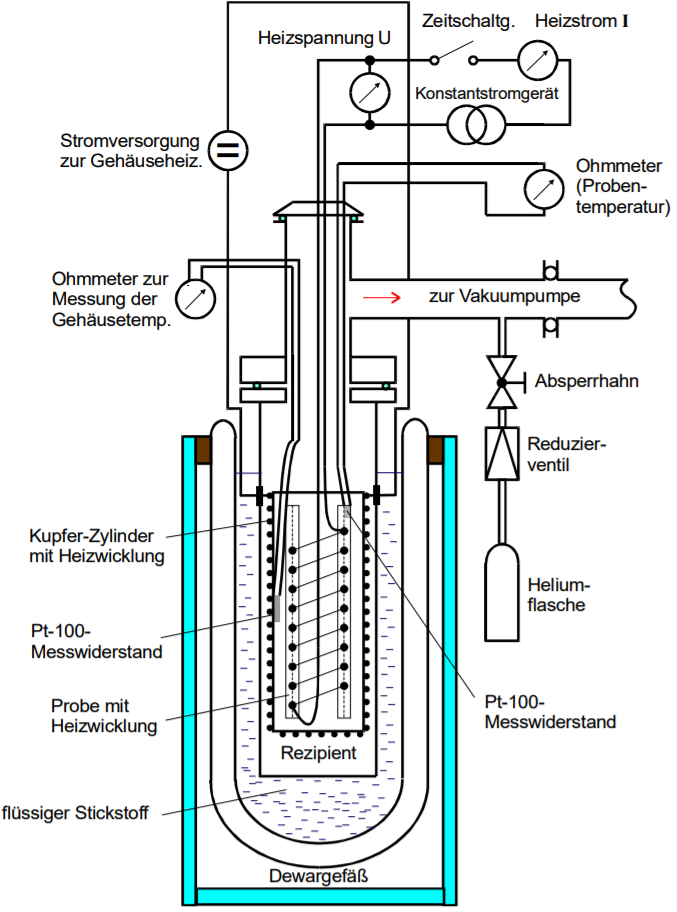
\includegraphics[width=0.7\textwidth]{Bilder/aufbau.png}
  \caption{Aufbau des Experiments.\cite{anleitung}}
  \label{fig:aufbau}
\end{figure}

Die $\gamma$-Strahlungsquelle $\ce{^{137}Cs}$ ist fest im Aufbau installiert. Um die Strahlung möglichst parallel auf den Würfel treffen zu lassen, wird direkt vor der Quelle die Strahlung durch ein
kleines Loch in einer Bleiplatte abgeschirmt und somit kollimiert.
Im Strahlengang ist eine Möglichkeit gegeben, den Würfel beweglich zu platzieren.
Nach Abschirmung durch den Würfel trifft die verbleibende Strahlung auf einen Szintillationsdetektor.
Dieser besteht aus einem anorganischen Szintillator und einem Photomultiplier.
Durch die Bestrahlung wird der Szintillator angeregt und sendet im gleichen Verhältnis zu der eintreffenden Strahlung, Lichtblitze aus.
Diese emittierten Photonen treffen auf eine Photokathode, aus der durch den Photoeffekt Elektronen herausgelöst werden.
Diese werden schließlich im Photomultiplier vervielfacht und das entstandene elektrische Signal vom Multichannelanalyser ausgelesen.\\
Untersucht wird die mittlere Schicht eines Würfels, der sich insgesamt aus 3x3x3 Elementarwürfeln zusammensetzt; somit wird eine 3x3 Ebene untersucht.
Abbildung $\ref{fig:richtung}$ zeigt, die ausgewählten Projektionsrichtungen der Messreihen.
\clearpage
\section{Versuchsdurchführung}
Der Messablauf besteht aus einem Einsetzen des zu bemessenden Würfels, sodass der Strahl die gewünschte Richtung des Würfels durchläuft.
Danach wird die Zeitnahme gestartet und mit einem Computerprogramm die Messdaten des Szintillatorzählers ausgewertet.
Zu Anfang wird eine Messung der Nullrate durchgeführt, um am Ende einen Vergleichswert zu haben und etwaige äußere Umwelteinflüsse für die Auswertung berücksichtigen zu können.
Auch sind die zu vermessenden Würfel von einem Aluminiumgitter umschlossen, das auch seperat vermessen wird.
Es dient dazu, $\beta$-Strahlung abzuschirmen und nur die $\gamma$-Strahlung durchzulassen.
Da es Ziel des Versuchs ist mit der Tomographie einen vom Material her unbekannten Würfel zu analysieren, wird
als Vergleichsmessung je ein Würfel komplett aus Blei und Aluminium vermessen.
Da die Materialzusammensetzung dieser Würfel bekannt ist und angenommen werden kann, dass die Zusammensetzung homogen ist, werden 4 bis 5 Messungen pro Probe durchgeführt.
Schließlich folgt die genauere Messung mit 12 Raumrichtungen des unbekannten Würfels.
Die Projektionsrichtungen sind in Abbildung \ref{fig:richtung} zu sehen.
\begin{figure}[H]
  \centering
  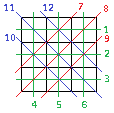
\includegraphics[width=0.5\textwidth]{Bilder/richtung.png}
  \caption{Messrichtungen der Projektion.}
  \label{fig:richtung}
\end{figure}
Damit der statistische Poissonfehler für die Auswertung vernachlässigt werden kann,
wird die Anzahl der Zähler mit
\begin{equation}
  \frac{1}{\sqrt{N}}<0,003
\end{equation}
abgeschätzt.
Es ergibt sich eine Mindestzahl für die Zähler von 1112. Außerdem wird für eine Projektionsrichtung eine Messzeit von mindestens $\SI{60}{s}$ angenommen.
Lediglich für die Bleizusammensetzung werden aufgrund des hohen Absorptionsvermögens circa $\SI{300}{s}$ gemessen.
